%%%%%%%%%%%%%%%%%%%%%%%%%%%%%%%%%%%%%%%%%
% Programming/Coding Assignment
% LaTeX Template
%
% This template has been downloaded from:
% http://www.latextemplates.com
%
% Original author:
% Ted Pavlic (http://www.tedpavlic.com)
%
% Note:
% The \lipsum[#] commands throughout this template generate dummy text
% to fill the template out. These commands should all be removed when 
% writing assignment content.
%
% This template uses a Perl script as an example snippet of code, most other
% languages are also usable. Configure them in the "CODE INCLUSION 
% CONFIGURATION" section.
%
%%%%%%%%%%%%%%%%%%%%%%%%%%%%%%%%%%%%%%%%%

%----------------------------------------------------------------------------------------
%	PACKAGES AND OTHER DOCUMENT CONFIGURATIONS
%----------------------------------------------------------------------------------------

%\documentclass{article}
\documentclass[12pt]{article}
\usepackage{fancyhdr} % Required for custom headers
\usepackage{lastpage} % Required to determine the last page for the footer
\usepackage{extramarks} % Required for headers and footers
\usepackage[usenames,dvipsnames]{color} % Required for custom colors
\usepackage{graphicx} % Required to insert images
\usepackage{subcaption}
\usepackage{listings} % Required for insertion of code
\usepackage{courier} % Required for the courier font
\usepackage{amsmath}
\usepackage{framed}

% Margins
\topmargin=-0.45in
\evensidemargin=0in
\oddsidemargin=0in
\textwidth=6.5in
\textheight=9.0in
\headsep=0.25in

\linespread{1.1} % Line spacing

% Set up the header and footer
\pagestyle{fancy}
\lhead{\hmwkAuthorName} % Top left header
\chead{\hmwkClass\ (\hmwkClassTime): \hmwkTitle} % Top center head
%\rhead{\firstxmark} % Top right header
\lfoot{\lastxmark} % Bottom left footer
\cfoot{} % Bottom center footer
\rfoot{Page\ \thepage\ of\ \protect\pageref{LastPage}} % Bottom right footer
\renewcommand\headrulewidth{0.4pt} % Size of the header rule
\renewcommand\footrulewidth{0.4pt} % Size of the footer rule

\setlength\parindent{0pt} % Removes all indentation from paragraphs

%----------------------------------------------------------------------------------------
%	CODE INCLUSION CONFIGURATION
%----------------------------------------------------------------------------------------

\definecolor{mygreen}{rgb}{0,0.6,0}
\definecolor{mygray}{rgb}{0.5,0.5,0.5}
\definecolor{mymauve}{rgb}{0.58,0,0.82}

\lstset{ %
  backgroundcolor=\color{white},   % choose the background color
  basicstyle=\footnotesize,        % size of fonts used for the code
  breaklines=true,                 % automatic line breaking only at whitespace
  captionpos=b,                    % sets the caption-position to bottom
  commentstyle=\color{mygreen},    % comment style
  escapeinside={\%*}{*)},          % if you want to add LaTeX within your code
  keywordstyle=\color{blue},       % keyword style
  stringstyle=\color{mymauve},     % string literal style
}

%----------------------------------------------------------------------------------------
%	DOCUMENT STRUCTURE COMMANDS
%	Skip this unless you know what you're doing
%----------------------------------------------------------------------------------------

% Header and footer for when a page split occurs within a problem environment
\newcommand{\enterProblemHeader}[1]{
%\nobreak\extramarks{#1}{#1 continued on next page\ldots}\nobreak
%\nobreak\extramarks{#1 (continued)}{#1 continued on next page\ldots}\nobreak
}

% Header and footer for when a page split occurs between problem environments
\newcommand{\exitProblemHeader}[1]{
%\nobreak\extramarks{#1 (continued)}{#1 continued on next page\ldots}\nobreak
%\nobreak\extramarks{#1}{}\nobreak
}

\setcounter{secnumdepth}{0} % Removes default section numbers
\newcounter{homeworkProblemCounter} % Creates a counter to keep track of the number of problems
\setcounter{homeworkProblemCounter}{0}

\newcommand{\homeworkProblemName}{}
\newenvironment{homeworkProblem}[1][Part \arabic{homeworkProblemCounter}]{ % Makes a new environment called homeworkProblem which takes 1 argument (custom name) but the default is "Problem #"
\stepcounter{homeworkProblemCounter} % Increase counter for number of problems
\renewcommand{\homeworkProblemName}{#1} % Assign \homeworkProblemName the name of the problem
\section{\homeworkProblemName} % Make a section in the document with the custom problem count
\enterProblemHeader{\homeworkProblemName} % Header and footer within the environment
}{
\exitProblemHeader{\homeworkProblemName} % Header and footer after the environment
}

\newcommand{\problemAnswer}[1]{ % Defines the problem answer command with the content as the only argument
\noindent\framebox[\columnwidth][c]{\begin{minipage}{0.98\columnwidth}#1\end{minipage}} % Makes the box around the problem answer and puts the content inside
}

\newcommand{\homeworkSectionName}{}
\newenvironment{homeworkSection}[1]{ % New environment for sections within homework problems, takes 1 argument - the name of the section
\renewcommand{\homeworkSectionName}{#1} % Assign \homeworkSectionName to the name of the section from the environment argument
\subsection{\homeworkSectionName} % Make a subsection with the custom name of the subsection
\enterProblemHeader{\homeworkProblemName\ [\homeworkSectionName]} % Header and footer within the environment
}{
\enterProblemHeader{\homeworkProblemName} % Header and footer after the environment
}

%----------------------------------------------------------------------------------------
%	NAME AND CLASS SECTION
%----------------------------------------------------------------------------------------

\newcommand{\hmwkTitle}{Programming Assignment 4} % Assignment title
\newcommand{\hmwkDueDate}{Thrusday, Mar 29, 2019} % Due date
\newcommand{\hmwkClass}{CSC421} % Course/class
\newcommand{\hmwkClassTime}{LEC 5101} % Class/lecture time
\newcommand{\hmwkAuthorName}{Zhongtian Ouyang} % Your name
\newcommand{\hmwkAuthorID}{1002341012} % Your ID


%----------------------------------------------------------------------------------------
%	TITLE PAGE
%----------------------------------------------------------------------------------------

\title{
\vspace{2in}
\textmd{\textbf{\hmwkClass:\ \hmwkTitle}}\\
\normalsize\vspace{0.1in}\small{Due\ on\ \hmwkDueDate}\\
\vspace{0.1in}
\vspace{3in}
}

\author{\textbf{\hmwkAuthorName}\\ \textbf{\hmwkAuthorID}}

\date{} % Insert date here if you want it to appear below your name

%----------------------------------------------------------------------------------------\
\begin{document}

\maketitle
\clearpage

%----------------------------------------------------------------------------------------
%	Common Tools
%----------------------------------------------------------------------------------------
%\begin{framed}
%\begin{lstlisting}[language=matlab]
%\end{lstlisting}
%\end{framed}

% \begin{bmatrix}
%0.5 & 0.6 \\ 
%0.7 & 0.8
%\end{bmatrix}

%\begin{figure}[h!]
%\centering
%\includegraphics[width=0.6\linewidth]{q10a.png}
%\label{fig:q10a}
%\end{figure}\\

%\begin{figure*}[!ht]
%\begin{subfigure}{.5\textwidth}
% \centering
%  \includegraphics[width=.5\linewidth]{p4_1.JPG}
%  \caption{Full set}
%  \label{fig:sfig1}
%\end{subfigure}
%\begin{subfigure}{.5\textwidth}
% \centering
%  \includegraphics[width=.5\linewidth]{P4_2.JPG}
%  \caption{Two each}
%  \label{fig:sfig2}
%\end{subfigure}%
%\caption{Part4 (a)}
%\label{fig:p4a}
%\end{figure*}

%\sum_{n=1}^{\infty} 2^{-n} = 1
%\prod_{i=a}^{b} f(i)
%----------------------------------------------------------------------------------------
%	PROBLEM 1
%----------------------------------------------------------------------------------------

% To have just one problem per page, simply put a \clearpage after each problem
\begin{homeworkProblem}
\noindent \textit{Deep Convolutional GAN}\\

1. \\
Let input width = W, output width = 0.5W:\\
Using the formula from csc411:
$$0.5W = \frac{W - F + 2P}{S} + 1 = \frac{W - 5 + 2P}{2} + 1 = 0.5W - 2.5 + P + 1,\ P = 1.5 \approx 2$$
The zero padding should be 2.\\

2.\\
The following samples are from iteration 200 and iteration 4000. The quality for both images are not very ideal. An human can easily identify this emojis as generated since they have serious artifacts. However, the quality does improve a lot through the training process. Compare to the one from iteration 200, where all the generated emojis look like some random pixels, the one from iteration 4000 have some emojis that are recognizable such as a face or a human. Both the shape and the color of the emojis improved a lot.
\begin{figure*}[!ht]
\begin{subfigure}{.5\textwidth}
 \centering
  
\includegraphics[width=\linewidth]{sample-000200.png}
  \caption{Iteration 200}
\end{subfigure}
\begin{subfigure}{.5\textwidth}
 \centering
  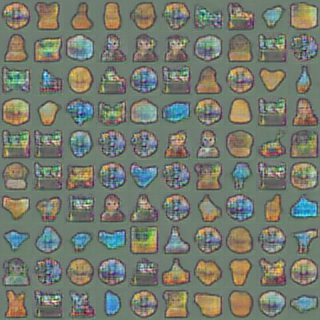
\includegraphics[width=\linewidth]{sample-004000.png}
  \caption{Iteration 4000}
\end{subfigure}
\end{figure*}
\end{homeworkProblem}
\clearpage
%----------------------------------------------------------------------------------------
%	PROBLEM 2
%----------------------------------------------------------------------------------------

\begin{homeworkProblem}
\noindent \textit{CycleGAN}\\

1.
\begin{figure*}[!ht]
\begin{subfigure}{.5\textwidth}
 \centering
  
\includegraphics[width=\linewidth]{sample-000200-X-Y.png}
  \caption{X to Y}
\end{subfigure}
\begin{subfigure}{.5\textwidth}
 \centering
  
\includegraphics[width=\linewidth]{sample-000200-Y-X.png}
  \caption{Y to X}
\end{subfigure}
\caption{Iteration 200}
\end{figure*}
\begin{figure*}[!ht]
\begin{subfigure}{.5\textwidth}
 \centering
  
\includegraphics[width=\linewidth]{sample-010000-X-Y.png}
  \caption{X to Y}
\end{subfigure}
\begin{subfigure}{.5\textwidth}
 \centering
  
\includegraphics[width=\linewidth]{sample-010000-Y-X.png}
  \caption{Y to X}
\end{subfigure}
\caption{Iteration 10000}
\end{figure*}

2.\\
The most noticible difference is the colour of the generated images. In one of the random seeds I tried, the green and red channel in the generated images seems to be switched. And the other random seeds also result in slightly differently colored generated images. The reason is that with different random seeds, the neural net is trained to different local min. Since the color of the content of an emoji (except the black edge for windows emojis) doesn't really affect how the discriminator decide whether it is a generated or original emoji, and since the difference in color can be reverted when translating the emoji back as long as the contrast information is preserved, neural networks with different initial weights will generate differently colored emojis.\\

3.\\
Using 4 as the random seed. For lambda\_cycle = 0.015, same as the above in Q1.\\
When lambda\_cycle = 0:
\begin{figure*}[!ht]
\begin{subfigure}{.5\textwidth}
 \centering
  
\includegraphics[width=\linewidth]{sample-000200-X-Y (4).png}
  \caption{X to Y}
\end{subfigure}
\begin{subfigure}{.5\textwidth}
 \centering
  
\includegraphics[width=\linewidth]{sample-000200-Y-X (4).png}
  \caption{Y to X}
\end{subfigure}
\caption{Iteration 200}
\end{figure*}
\begin{figure*}[!ht]
\begin{subfigure}{.5\textwidth}
 \centering
  
\includegraphics[width=\linewidth]{sample-010000-X-Y (4).png}
  \caption{X to Y}
\end{subfigure}
\begin{subfigure}{.5\textwidth}
 \centering
  
\includegraphics[width=\linewidth]{sample-010000-Y-X (4).png}
  \caption{Y to X}
\end{subfigure}
\caption{Iteration 10000}
\end{figure*}

These samples from a CycleGAN neural net trained without the cycle-consistency loss are very different from the previous results.. With lambda\_cycle = 0, the generated emojis doen't preserve the shape and color of the original emoji well because the NN is not penalized for not being able to translate the emojis back to the original.
\clearpage

When lambda\_cycle = 0.1:
\begin{figure*}[!ht]
\begin{subfigure}{.5\textwidth}
 \centering
  
\includegraphics[width=\linewidth]{sample-000200-X-Y (5).png}
  \caption{X to Y}
\end{subfigure}
\begin{subfigure}{.5\textwidth}
 \centering
  
\includegraphics[width=\linewidth]{sample-000200-Y-X (5).png}
  \caption{Y to X}
\end{subfigure}
\caption{Iteration 200}
\end{figure*}
\begin{figure*}[!ht]
\begin{subfigure}{.5\textwidth}
 \centering
  
\includegraphics[width=\linewidth]{sample-010000-X-Y (5).png}
  \caption{X to Y}
\end{subfigure}
\begin{subfigure}{.5\textwidth}
 \centering
  
\includegraphics[width=\linewidth]{sample-010000-Y-X (5).png}
  \caption{Y to X}
\end{subfigure}
\caption{Iteration 10000}
\end{figure*}

When lambda\_cycle = 0.1, the shape of the generated emojis are almost identical to the original emoji, while the color are very different. The reason is that with a large lambda\_cycle, the NN is penalized hard for failing to translate the emojis back to the original and therefore, it choose to prioritize this function more. To do so, preserving the shape is very important. As a comparison, as explained in Q2, the color of generated emoji doesn't really matter as long as the color mapping information is captured in the weights.
\end{homeworkProblem}
\clearpage
%----------------------------------------------------------------------------------------

\end{document}
